\graphicspath{{./lib/ti_amplifier/figures/}}
\clearpage
\section{TI Amplifier}
\begin{tcolorbox}	
	\begin{tabular}{p{2.75cm} p{0.2cm} p{10.5cm}} 	
		\textbf{Header File}   &:& Ti\_amplifier.h \\
		\textbf{Source File}   &:& ti\_amplifier.cpp \\
		\textbf{Version}       &:& 20190327\\
		\textbf{Version}       &:& 20190327 (Bruno Santos 79965)\\
	\end{tabular}
\end{tcolorbox}
\maketitle
In practically almost all RF receivers we have an \textit{amplifier} that gives power to the signal coming from the antenna. Since our received power is very low we must have big gain and low noise to try not to change the SNR in order to minimize the BER. \newline
This block has the function of converting and amplifying the signal that comes from the photodetectors. It has an input signal and an output which is the product of the input signal, added with white noise and then filtered by a Low-Pass filter. This way we can simulate a real transipedance amplifier and change its electrical characteristics.


\subsection*{Input Parameters}

\begin{itemize}
	\item rxTiAmplifierInputNoisePowerSpectralDensity(0) :  Modulate the PSD of the white noise generated by the block
	\item rxTiAmplifierImpulseResponseTimeLengthsymbolPeriods(20) : Used to change the time length response of the amplifier filter
	\item rxTiAmplifierBandwith(50e9) : Change the cutoff frequency of the Low pass filter
\end{itemize}


\subsection*{Input Signals}
\subparagraph*{Number:} 6 and 7 Balanced Photodetectors
\subparagraph*{Type:} Optical Signal (TimeContinuousAmplitudeContinuousReal)
\subsection*{Output Signals}
\subparagraph*{Number:} 8 and 9 Ti\textunderscore Amplifier Output
\subparagraph*{Type:} Electrical (TimeContinuousAmplitudeContinuousReal)
\subsection*{Internal Signals}
\subparagraph*{\texttt{White Noise}}
\texttt{Type:} Eletrical (TimeContinuousAmplitudeContinuousReal)
\subparagraph*{\texttt{Add}}
\texttt{Type:} Eletrical (TimeContinuousAmplitudeContinuousReal)
\subparagraph*{\texttt{Ideal Amplifier}}
\texttt{Type:} Eletrical (TimeContinuousAmplitudeContinuousReal)
\subparagraph*{\texttt{Electrical Filter}}
\texttt{Type:} Eletrical (TimeContinuousAmplitudeContinuousReal)

\subsection*{Methods}
TiAmplifier(initializer\textunderscore List<Signal *> inputSignals, initializer\textunderscore list<Signal *> outputSignals) : SuperBlock(inputSignals, outputSignals) {};
\bigbreak
\begin{itemize}
    \item void setInputReferredNoisePowerSpectralDensity(double newInputReferredNPDS)
    \item void setNoiseSamplingPeriod(t\textunderscore real samplingPeriod)
    \item void setNoiseSymbolPeriod(t\textunderscore real symPeriod)
    \item void setGain(double ga)
    \item void setFilterType(Filter filterType)
    \item void setCutoffFrequency(double cutoffFreq)
    \item void setImpulseResponseTimeLength()
    \item void setImpulseResponse(vector<t\textunderscore real> ir)
    \item void setImpulseResponseFilename(string fName)
    \item void setImpulseResponseLength(int impResponseLength)
    \item void setSeeBeginningOfImpulseResponse(bool sBegginingOfImpulseResponse)
\end{itemize}


\subsection{Examples}
\paragraph*{} In this section we will see some examples of the signals present in this super block and the cause-effect of variations in the electrical characteristics such as Noise power or the cuttoff frequency.
\begin{figure}
	\centering
	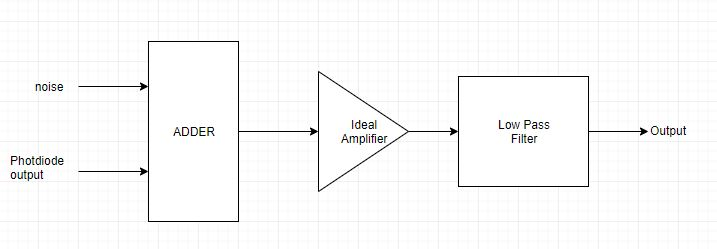
\includegraphics{diagram.png}
	\caption{The block diagram of TI amplifier super block}
	\label{fig:blocks}
\end{figure}

\begin{figure}%
	\begin{subfigure}[h]{0.4\textwidth}
		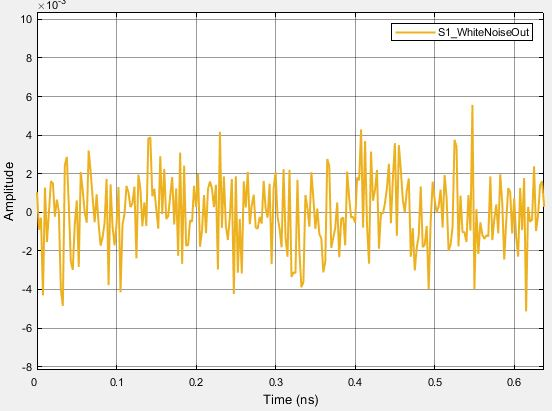
\includegraphics[scale=0.45]{white_noise_in.png}
		\caption{The white noise generated by the electrical elements and the electrical signal coming from the photodetectors}
		\label{fig:White Noise}
	\end{subfigure}
	\begin{subfigure}[h]{0.4\textwidth}
		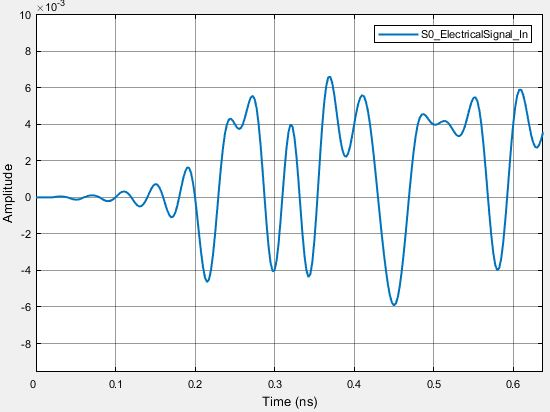
\includegraphics[scale=0.45]{Electrical_signal_in.png}
		\caption{Electrical signal at input of adder block}
		\label{fig:Adder In}
	\end{subfigure}
	\centering
	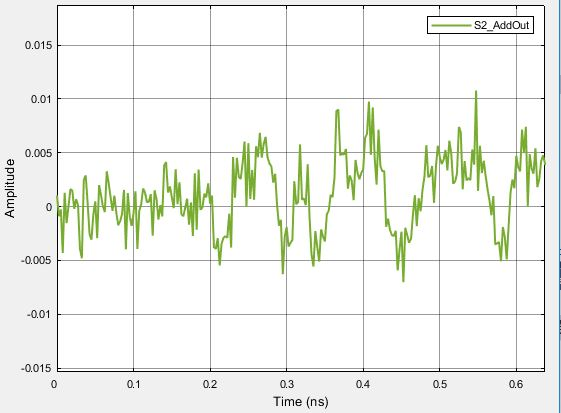
\includegraphics[scale=0.45]{adder_out.png}
	\caption{Output signal of the adder block which is the sum of white noise with the electrical signal}
	\label{fig:Adder Out}
\end{figure}
\begin{figure}
	\centering
	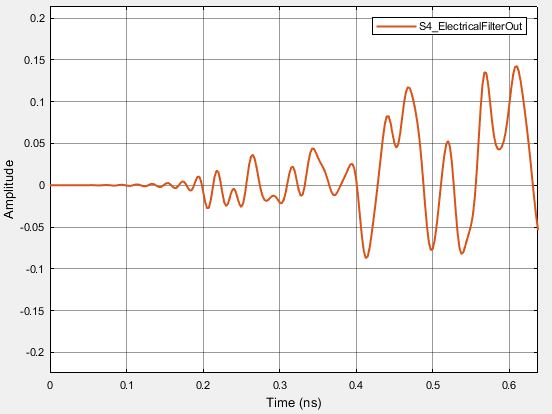
\includegraphics[scale=0.45]{filter_out.png}
	\caption{The output of the TI Amplifier after being filtered by a low pass}
	\label{fig:TI_out}
\end{figure}


\subsection*{Functional description}
\begin{text}
The transipedance amplifier can be split into three minor blocks in order to simulate a real amplifier as we can see in \ref{fig:blocks}
\newline
\subsection{Adder Block:} in this stage we simulate the noise generated by the electrical components of the real amplifier. Since the noise has a gaussian distribution we consider it as white noise. In the above examples we can see the output of this block which is the sum of the signal with the noise. See \ref{fig:Adder Out}

\subsection{Ideal Amplifier:} This block converts the current signal into voltage and add power to the signal. After this stage the SNR of this signal is slightly reduced by the effect of the previous block.\newline

\subsection{Low Pass Filter:} All real amplifiers are non linear and it's transfer function is characterized by being approximately a low pass filter. In this case, our input has frequency content until infinite because of the white noise and our real amplifier can't give power to all frequencies. In the examples, in the \ref{fig:TI_out} it is possible to see that the high frequency noise is filtered.
\end{text}
\pagebreak

\subsection*{Suggestions for future improvement}
